\documentclass{article}%
\usepackage[T1]{fontenc}%
\usepackage[utf8]{inputenc}%
\usepackage{lmodern}%
\usepackage{textcomp}%
\usepackage{lastpage}%
\usepackage[head=40pt,margin=0.5in,bottom=0.6in]{geometry}%
\usepackage{graphicx}%
%
\title{\textbf{Familiares denuncian que funcionarios de PNB engañaron a presos colombianos}}%
\author{RAFAEL LEÓN | raleon@el{-}nacional.com}%
\date{05/12/2018}%
%
\begin{document}%
\normalsize%
\maketitle%
\textbf{URL: }%
http://www.el{-}nacional.com/noticias/politica/familiares{-}denuncian{-}que{-}funcionarios{-}pnb{-}enganaron{-}presos{-}colombianos\_262158\newline%
%
\textbf{Periodico: }%
EN, %
ID: %
262158, %
Seccion: %
Política\newline%
%
\textbf{Palabras Claves: }%
NO\_TIENE\newline%
%
\textbf{Derecho: }%
1.2, %
Otros Derechos: %
1.10, %
Sub Derechos: %
1.2.2, 1.10.1\newline%
%
\textbf{EP: }%
NO\newline%
\newline%
%
\textbf{\textit{Los agentes les habían prometido la libertad si firmaban un documento, el cual suscribieron antes de la audiencia y sin presencia de sus abogados}}%
\newline%
\newline%
%
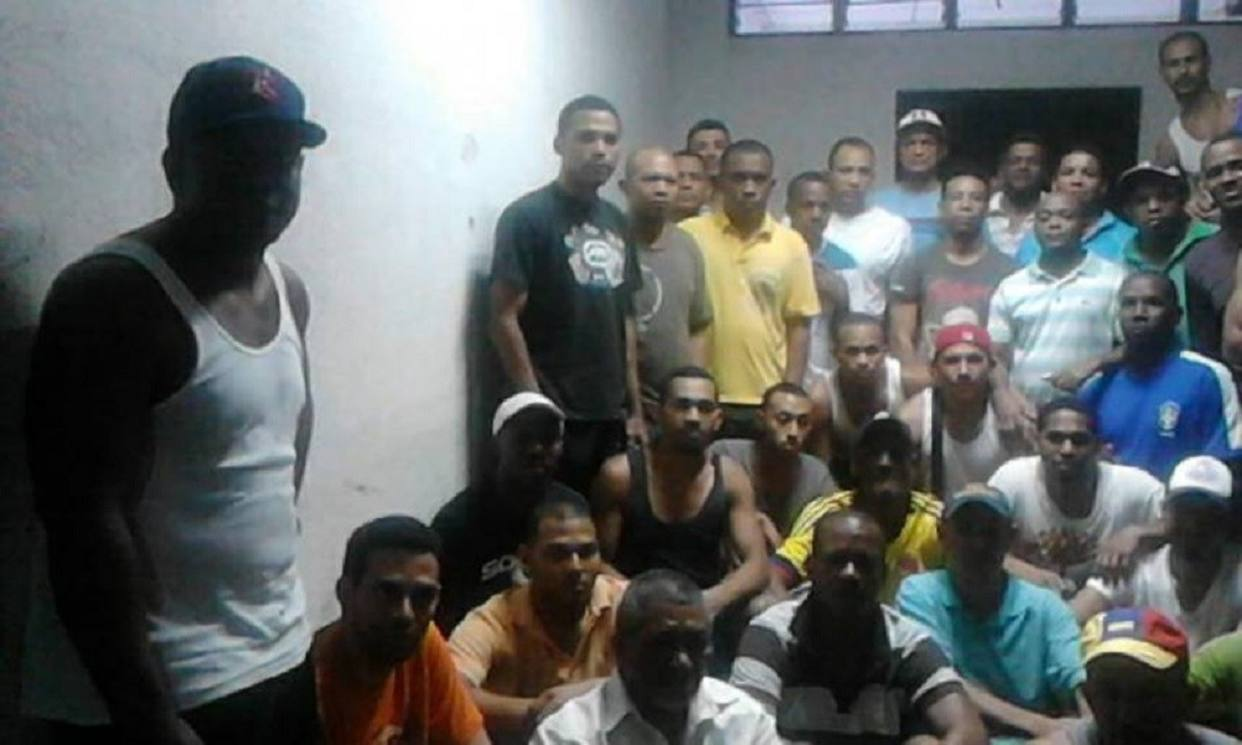
\includegraphics[width=300px]{217.jpg}%
\newline%
%
Los 59 colombianos detenidos en Venezuela desde 2016 por delitos migratorios fueron engañados por funcionarios de~la Policía Nacional~Bolivariana de~La Yaguara, que~les prometieron liberarlos y deportarlos si firmaban un documento del cual desconocían el contenido, denunció un grupo de familiares que añadieron que luego de suscribir el escrito –sin presencia de sus abogados– los presentaron ante los tribunales y les imputaron tres cargos.%
\newline%
%
“Estamos comprobando que aquí en Venezuela no se respetan los derechos humanos ni el debido proceso. Los 59 colombianos están secuestrados por el gobierno”, manifestó Lisbeth Rivera, esposa de uno de los detenidos.%
\newline%
%
Señaló que el caso ha sido “una burla” para ellos debido a que luego de~más de dos años de encarcelamiento –sin orden de detención– por presuntos delitos migratorios, el 21 de noviembre los presentaron ante un tribunal especial constituido en la sede de~la PNB,~en~La Yaguara, no les permitieron la asistencia de sus abogados privados ni del Consulado de Colombia. Fueron imputados por terrorismo, instigación a delinquir y falsificación de documentos, a pesar de que el año pasado un tribunal de control ordenó excarcelarlos al considerar que no había orden de aprehensión ni evidencia de delito.%
\newline%
%
“Tememos por lo que pueda suceder con ellos porque no sabemos cuál es el propósito del gobierno de Venezuela”, expresó Rivera. Aseguró que el Estado no les ha respetado el derecho a la salud ni a la alimentación, debido a que en la sede policial les suministran comida descompuesta.%
\newline%
%
Indicó que todos los involucrados en el caso fueron aprehendidos arbitrariamente durante los Operativos de Liberación del Pueblo, en diferentes fechas y lugares.%
\newline%
%
Para Amnistía Internacional la revocatoria de la orden de libertad pone a esas personas en “grave riesgo” de que se postergue indefinidamente la privación de libertad, y que continúe la violación a sus garantías procesales y sus derechos a un juicio justo.%
\newline%
%
La ONG exigió al gobierno la liberación de los 59 extranjeros. Denunciaron que durante la reclusión han estado en graves condiciones de insalubridad “que atentan contra su dignidad”, pues han sido encarcelados en celdas improvisadas, sin acceso a agua potable y en ocasiones han dormido a la intemperie.%
\newline%
%
La fiscal Luisa Ortega Díaz, quien ha rechazado las jornadas de la OLP, denunció el caso ante la Corte Penal Internacional y responsabilizó de la “detención arbitraria” al presidente Nicolás Maduro, al ministro de Interior, Néstor Reverol, así como al director de la PNB, Franklin García, y al ex titular de ese cargo, Juan Romero.%
\newline%
%
En estos dos años de detención,~la Embajada~de Colombia ha enviado más de 94 notas verbales a~la Cancillería, Fiscalía, Defensoría del Pueblo, Ministerio Interior y Justicia, al Saime, entre otros, y hasta la fecha no han recibido respuesta.~La semana pasada denunciaron el caso en la oficina de Michelle Bachelet, alta comisionada para los Derechos Humanos de~la Organización de Naciones Unidas.%
\newline%
%
Sin garantías%
\newline%
%
Espacio Público exigió al Estado la libertad del periodista alemán Billy Six, detenido por el DGCIM el sábado 17 de noviembre en Paraguaná y enjuiciado en un tribunal militar por presunta rebelión, violación de zonas de seguridad y espionaje.%
\newline%
%
Six es uno de los ocho periodistas internacionales perseguidos por el gobierno, de acuerdo con el registro de la ONG. El Comité para la Protección de los Periodistas expresó su preocupación por el caso e informó que la oficina de prensa del Ministerio de Asuntos Exteriores de Alemania estaba al tanto del caso y que la Embajada, en Caracas, brindó su asistencia consular.%
\newline%
%
\end{document}